\chapter{Mengen en oplossen}\label{ch:g2:mixing-and-dissolving}

Er plonst een suikerklontje in een kopje hete thee. Een lepeltje roert,
het klontje valt uit elkaar, en even later is er niets meer van te zien:
de thee ziet er precies zo uit als daarvoor. Toch smaakt de thee nu zoet.
De suiker is niet weg --- hij zit verstopt in de thee. Dit hoofdstuk gaat
over dingen samenvoegen, en over de dingen die daarbij lijken te
verdwijnen.

\begin{omfigure}
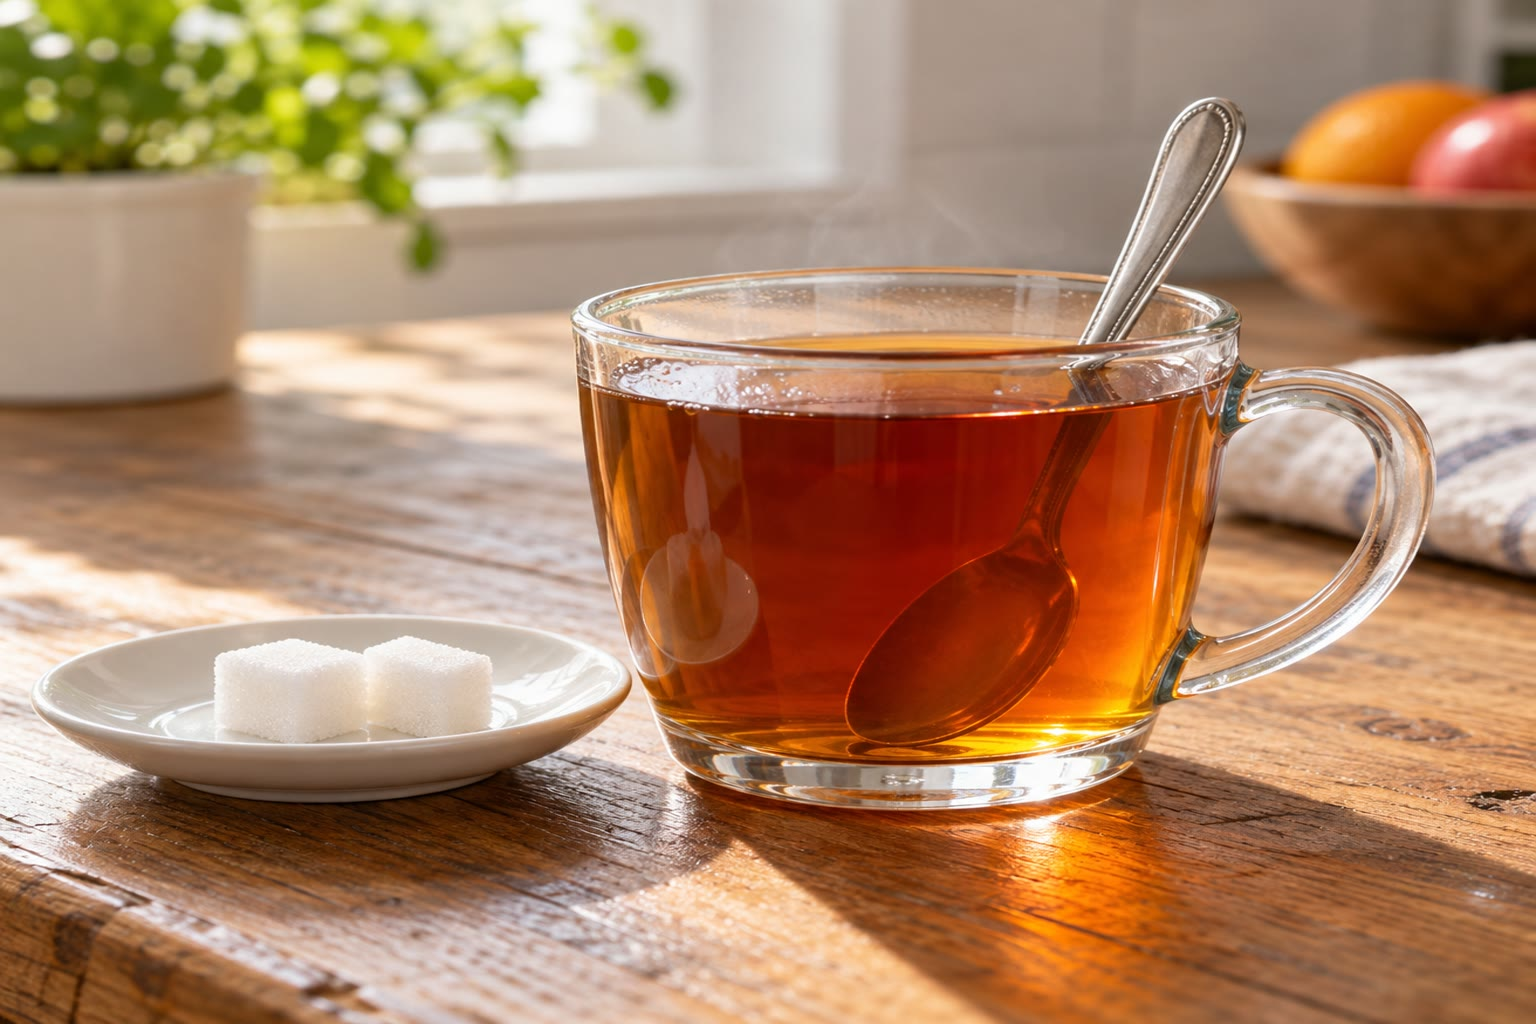
\includegraphics[width=0.55\linewidth]{images/book1/ai/g2-tea-sugar.jpg}

{\small Een kopje thee en twee suikerklontjes. Na het roeren is de suiker
niet meer te zien, maar wel te proeven.}
\end{omfigure}

\section{Dingen samen mengen}

\begin{definition}[Mengen]\label{def:g2:mixing-and-dissolving:mix}
\emph{Mengen}\index{mengen} is verschillende dingen bij elkaar doen, en
ze vaak ook door elkaar roeren. Wat we krijgen, is een mengsel van die
dingen.
\end{definition}

\begin{example}[Een kom muesli]\label{ex:g2:mixing-and-dissolving:muesli}
Havervlokken, rozijnen, noten en zaadjes gaan samen in één kom: dat is
een mengsel. Kijk goed: elk ingrediënt is nog te zien en kun je er met je
vingers weer uit halen --- een rozijn blijft een rozijn, een noot blijft
een noot.
\end{example}

\begin{example}[Siroop in water]\label{ex:g2:mixing-and-dissolving:syrup}
Ook twee vloeistoffen kun je \omterm{def:g2:mixing-and-dissolving:mix}{mengen}. Rode siroop die je in een glas water
giet, zakt naar beneden in kleurige krullen; na één keer roeren is het
hele glas gelijkmatig roze. Met het oog kun je de siroop en het water
niet meer uit elkaar houden.
\end{example}

\begin{omfigure}
\begin{minipage}[t]{0.48\linewidth}\centering
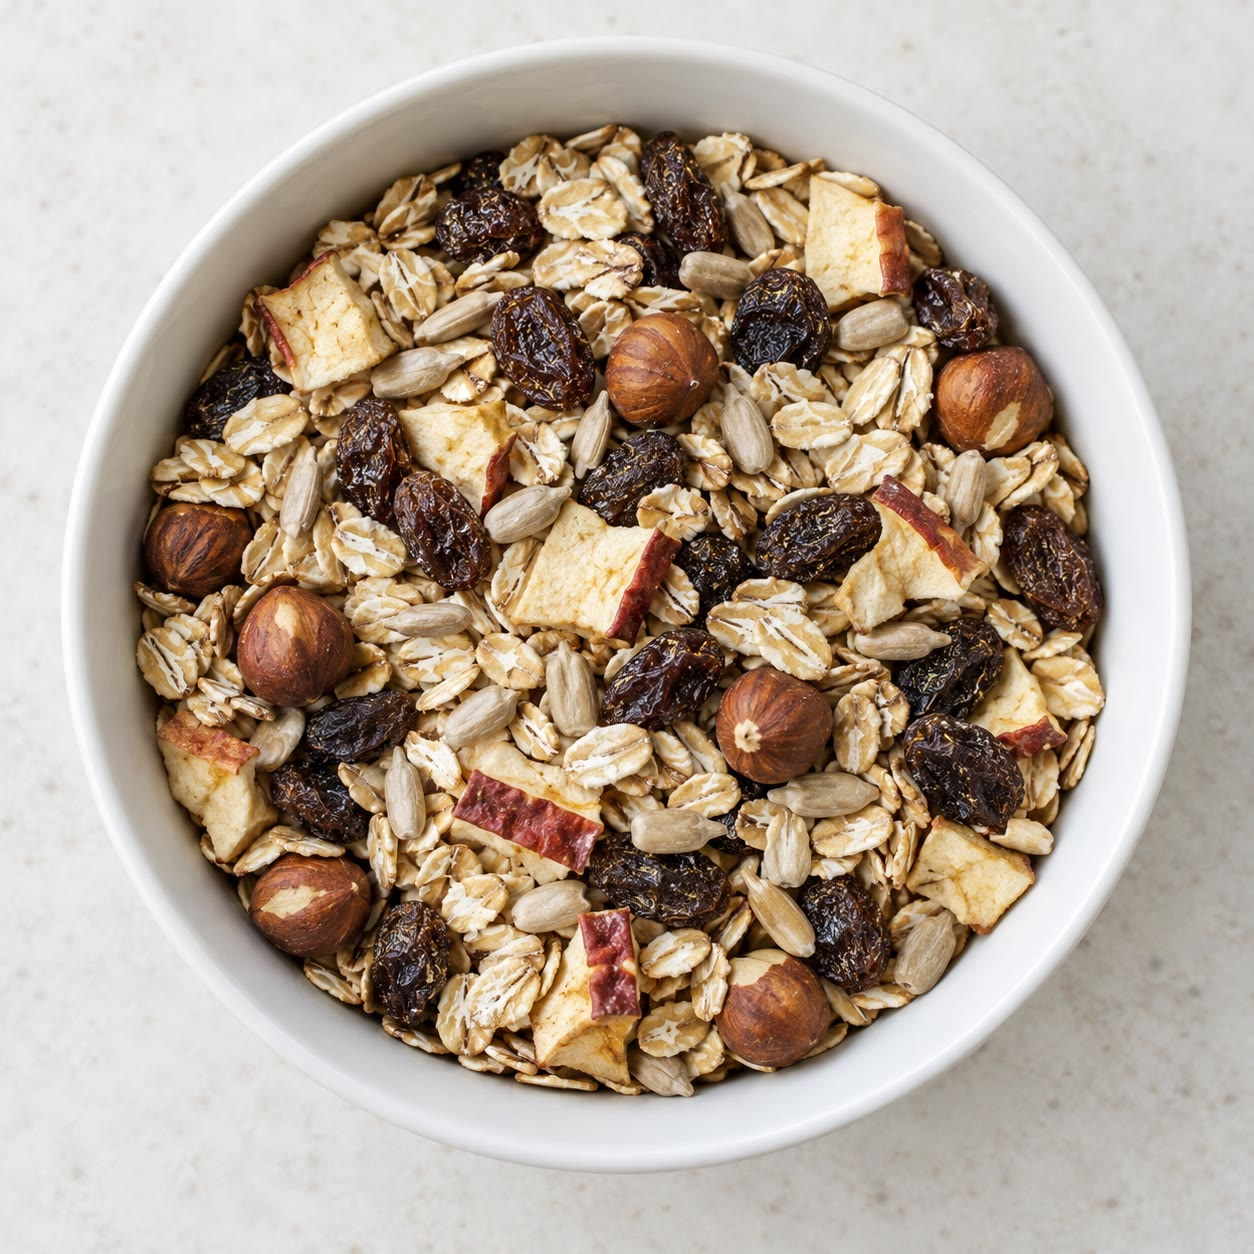
\includegraphics[width=\linewidth,height=4.6cm,keepaspectratio]{images/book1/ai/g2-muesli.jpg}

{\small Muesli: een mengsel waarin je elk deel nog kunt zien.}
\end{minipage}\hfill
\begin{minipage}[t]{0.48\linewidth}\centering
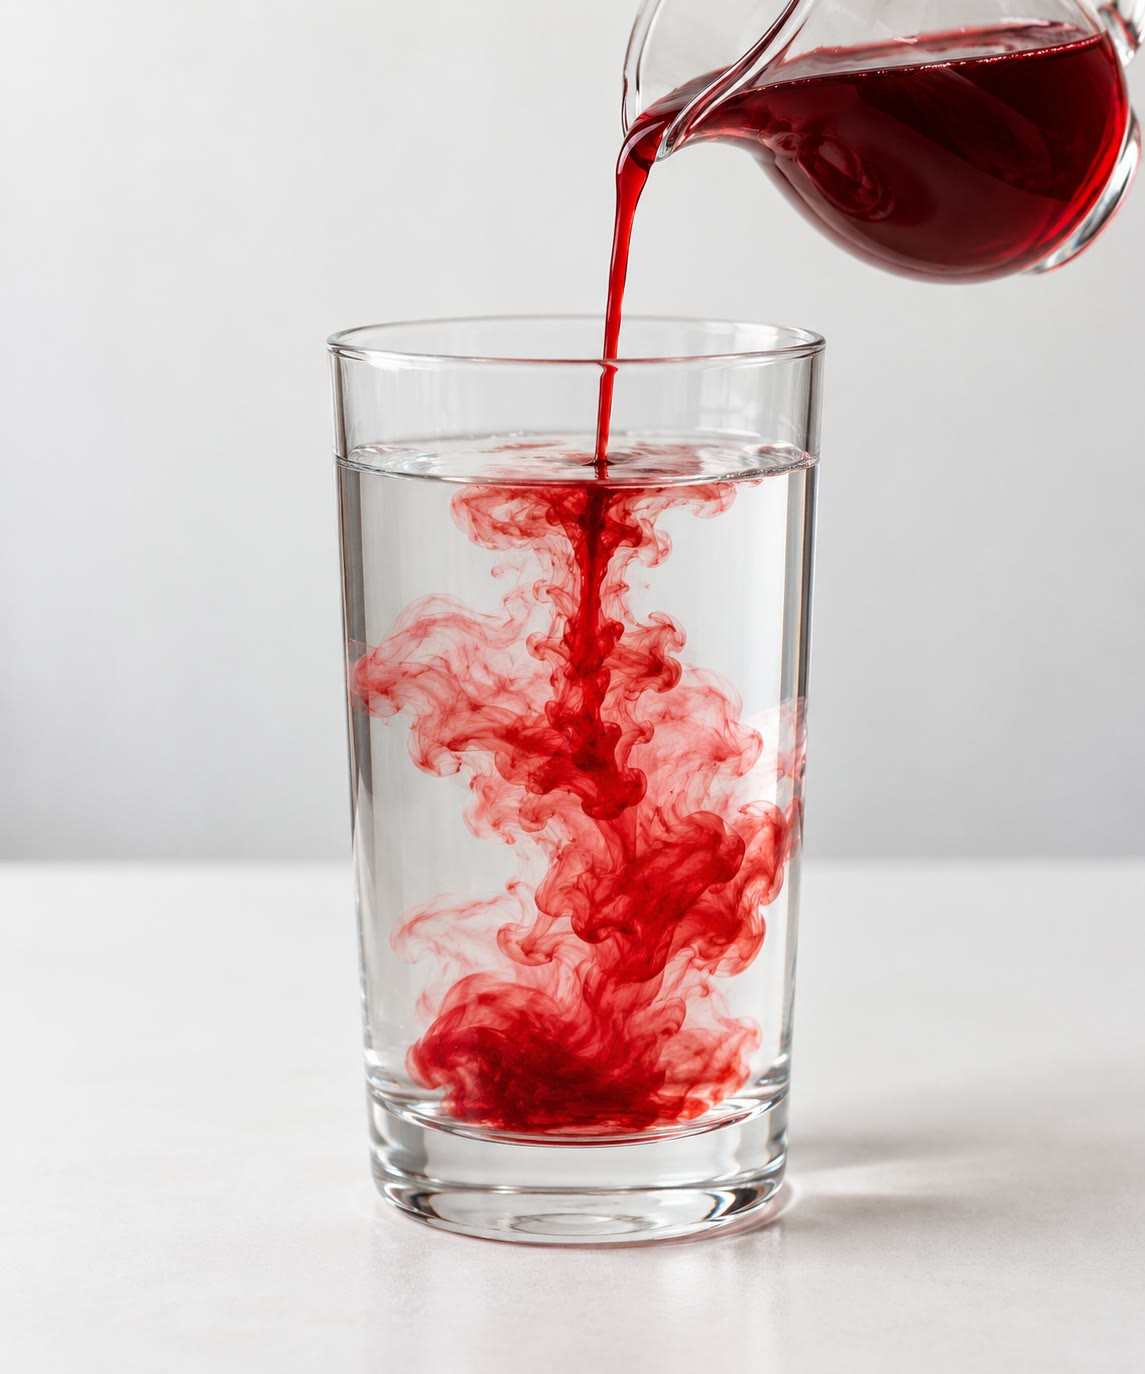
\includegraphics[width=\linewidth,height=4.6cm,keepaspectratio]{images/book1/ai/g2-syrup-in-water.jpg}

{\small Siroop in water gegoten: twee vloeistoffen die \omterm{def:g2:mixing-and-dissolving:mix}{mengen}.}
\end{minipage}
\end{omfigure}

\begin{remark}[Mengen maakt niets kapot]\label{rem:g2:mixing-and-dissolving:nothing-lost}
Als je dingen \omterm{def:g2:mixing-and-dissolving:mix}{mengt}, gaat er niets verloren en ontstaat er niets nieuws.
De havervlokken, de rozijnen en de noten zitten allemaal nog in de kom.
Een later hoofdstuk laat zien hoe je een mengsel weer uit elkaar haalt.
\end{remark}

\section{Dingen die oplossen}

\begin{definition}[Oplossen en oplossing]\label{def:g2:mixing-and-dissolving:dissolve}
Een vaste stof \emph{lost op}\index{oplossen} in water wanneer hij, door
het water geroerd, uit het zicht verdwijnt en de vloeistof
\emph{helder} laat, dat wil zeggen doorzichtig. Suiker en zout lossen op
in water. De heldere vloeistof die we zo krijgen, heet een
\emph{oplossing}\index{oplossing}: suikerwater is een oplossing van
suiker, zout water een oplossing van zout.
\end{definition}

\begin{example}[Een suikerklontje in een glas water]\label{ex:g2:mixing-and-dissolving:cube}
Een suikerklontje ligt op de bodem van een glas stilstaand water. De
hoekjes worden zacht, het klontje wordt kleiner, en er stijgen golvende
slierten van op door het water. Roeren we, dan is het binnen een minuut
weg. Roeren we niet, dan verdwijnt het ook, alleen veel langzamer.
\end{example}

\begin{remark}[Helder is niet hetzelfde als kleurloos]\label{rem:g2:mixing-and-dissolving:clear}
Thee is bruin en het siroopwater is roze, maar door allebei kunnen we
heen kijken: ze zijn helder. Een \omterm{def:g2:mixing-and-dissolving:dissolve}{oplossing} kan een kleur hebben. Wat een
\omterm{def:g2:mixing-and-dissolving:dissolve}{oplossing} nooit heeft, zijn stukjes die erin zweven of een laagje op de
bodem.
\end{remark}

\begin{method}[Lost het op?]\label{met:g2:mixing-and-dissolving:test}
Zo zoek je uit of een vaste stof in water \omterm{def:g2:mixing-and-dissolving:dissolve}{oplost}:
\begin{enumerate}
  \item doe een beetje van de vaste stof in een glas water;
  \item roer, en wacht dan een paar minuten;
  \item kijk door het glas:
    \begin{itemize}
      \item helder, en niets op de bodem: de vaste stof is opgelost;
      \item troebel, of een laagje op de bodem: de vaste stof is niet opgelost.
    \end{itemize}
\end{enumerate}
\end{method}

\section{Dingen die niet oplossen}

\begin{proposition}[Zand en krijt lossen niet op]\label{prop:g2:mixing-and-dissolving:not}
Veel vaste stoffen lossen niet op in water: zand, krijt, aarde, kiezels,
meel. Door water geroerd maken ze het troebel; laat je het staan, dan
zakken ze naar beneden en bezinken ze op de bodem, en het water erboven
wordt weer helderder. Hoe lang we ook roeren, ze verdwijnen nooit.
\end{proposition}

\begin{example}[Een pot modderwater]\label{ex:g2:mixing-and-dissolving:mud}
Tuinaarde die je in een pot water schudt, maakt het water bruin en
troebel. Na een uur liggen de aarde en de steentjes in een donkere laag
op de bodem, drijven er een paar dode blaadjes bovenop, en is het water
daartussen nog maar een beetje troebel. De aarde is niet opgelost.
\end{example}

\begin{omfigure}
\begin{minipage}[t]{0.48\linewidth}\centering
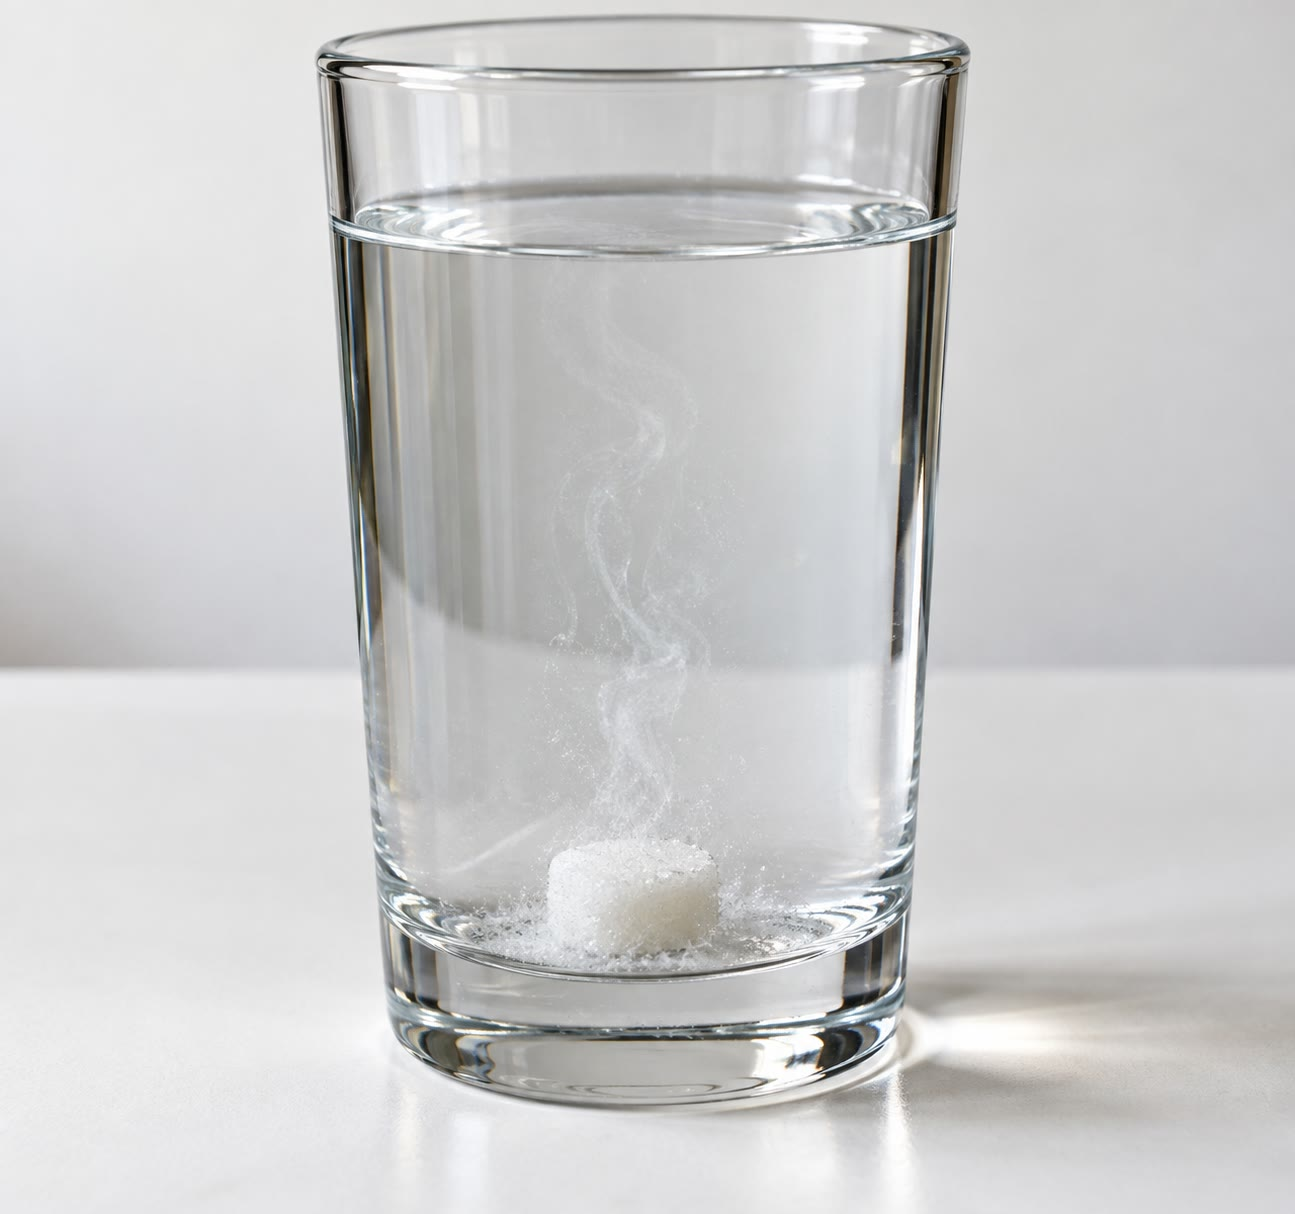
\includegraphics[width=\linewidth,height=4.6cm,keepaspectratio]{images/book1/ai/g2-sugar-cube-dissolving.jpg}

{\small Suiker \omterm{def:g2:mixing-and-dissolving:dissolve}{lost op}: er stijgen slierten op van het klontje.}
\end{minipage}\hfill
\begin{minipage}[t]{0.48\linewidth}\centering
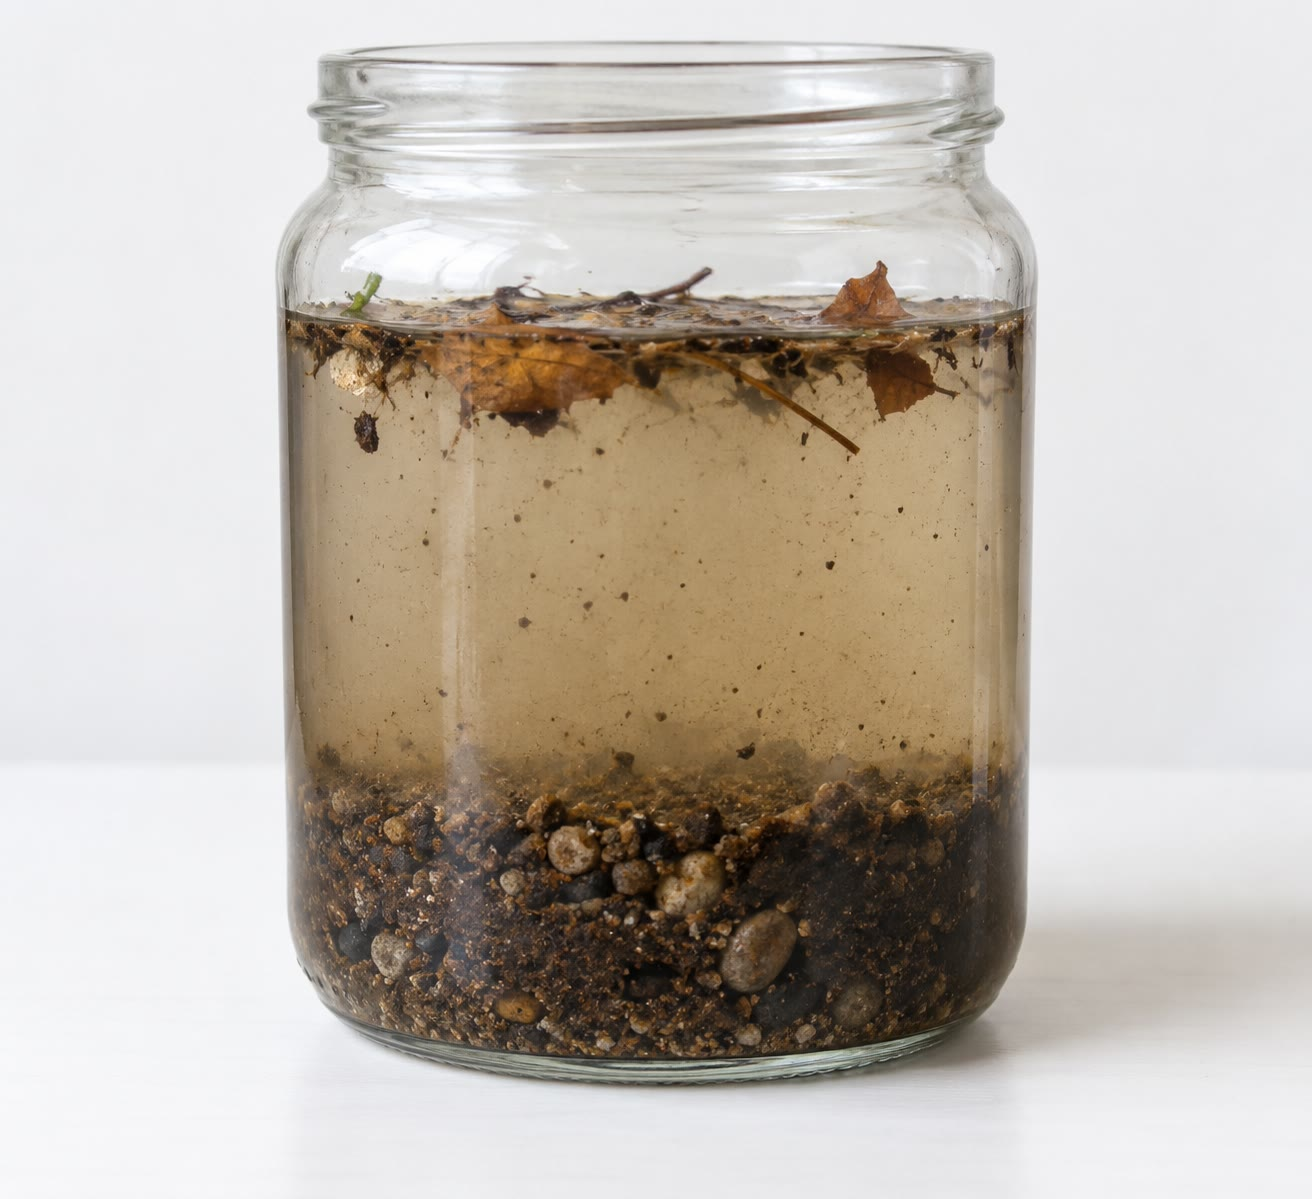
\includegraphics[width=\linewidth,height=4.6cm,keepaspectratio]{images/book1/ai/g2-muddy-jar.jpg}

{\small Aarde lost niet op: ze bezinkt op de bodem.}
\end{minipage}
\end{omfigure}

\begin{omfigure}
\begin{tikzpicture}[font=\small, scale=1.35]
  \pic[transform shape] at (0,0) {beaker={0.7}{omWater!70}};
  \fill[brown!55] (4.2,0) rectangle (5.8,0.22);
  \pic[transform shape] at (5,0) {beaker={0.7}{brown!12}};
  \fill[brown!55] (4.2,0) rectangle (5.8,0.22);
  \draw[omGlass, line width=0.7pt] (4.2,0.22) -- (4.2,0) -- (5.8,0) -- (5.8,0.22);
  \foreach \x/\y in {4.4/0.32,4.75/0.45,5.1/0.3,5.5/0.5,4.6/0.7,5.3/0.8,4.9/1.0}
    \fill[brown!60] (\x,\y) circle (0.025);
  \node[align=center, anchor=north] at (0,-0.15)
    {\textbf{suiker} in water, geroerd:\\ helder, niets op de bodem};
  \node[align=center, anchor=north] at (5,-0.15)
    {\textbf{zand} in water, geroerd:\\ troebel, een laagje op de bodem};
  \draw[<-, omProp, thick] (6.0,0.11) -- (7.0,0.11)
    node[right, text=black] {het zand};
\end{tikzpicture}

{\small De test van \cref{met:g2:mixing-and-dissolving:test}: suiker
\omterm{def:g2:mixing-and-dissolving:dissolve}{lost op}, zand niet.}
\end{omfigure}

\section{Wat oplost, is er nog}

\begin{proposition}[Een opgeloste vaste stof zit nog in het water]\label{prop:g2:mixing-and-dissolving:still-there}
Als een vaste stof \omterm{def:g2:mixing-and-dissolving:dissolve}{oplost}, verdwijnt hij niet: hij is door het hele
water verspreid, in stukjes die veel te klein zijn om te zien. Twee
aanwijzingen laten zien dat hij er nog is:
\begin{itemize}
  \item zoete thee smaakt zoet, en zeewater smaakt zout;
  \item als het water opdroogt, blijft de vaste stof achter.
\end{itemize}
\end{proposition}

\begin{remark}[In het laboratorium proef je niets]\label{rem:g2:mixing-and-dissolving:no-tasting}
We weten dat thee zoet is, omdat thee iets is wat we eten en drinken. In
een laboratorium proeft niemand ooit iets, ook geen vloeistof die eruitziet
als water: de tweede aanwijzing, het water laten opdrogen, is die welke
scheikundigen gebruiken.
\end{remark}

\begin{example}[Zout uit de zee]\label{ex:g2:mixing-and-dissolving:salt-pans}
Aan sommige zonnige kusten laat men zeewater in brede, ondiepe vijvers
lopen. Dag na dag laat de zon het water opdrogen. Wat er op de bodem
achterblijft, is wit zout, dat men tot hopen bijeenharkt: het zout dat in
de zee opgelost was. Het zout op de eettafel komt vaak uit zulke vijvers.
\end{example}

\begin{omfigure}
\begin{tikzpicture}[font=\small, scale=1.25]
  % day 1: a saucer of salty water
  \fill[omWater!80] (0,0.18) ellipse (1.25 and 0.22);
  \draw[omGlass, line width=0.7pt] (-1.5,0.3) .. controls (-1.2,-0.15) and (1.2,-0.15) .. (1.5,0.3);
  \draw[omGlass, line width=0.5pt] (0,0.3) ellipse (1.5 and 0.28);
  \node[align=center, anchor=north] at (0,-0.35) {een schoteltje\\ zout water};
  % the sun
  \fill[ocYellow] (3.4,1.45) circle (0.28);
  \foreach \a in {0,45,...,315}
    \draw[ocYellow!90!orange, thick] ($(3.4,1.45)+(\a:0.36)$) -- ($(3.4,1.45)+(\a:0.52)$);
  \draw[->, thick, omProp] (2.0,0.3) -- (4.8,0.3)
    node[midway, below, text=black, align=center] {een paar zonnige\\ dagen later};
  % later: a white crust
  \begin{scope}[xshift=6.3cm]
    \draw[omGlass, line width=0.7pt] (-1.5,0.3) .. controls (-1.2,-0.15) and (1.2,-0.15) .. (1.5,0.3);
    \draw[omGlass, line width=0.5pt] (0,0.3) ellipse (1.5 and 0.28);
    \foreach \x/\y in {-0.9/0.12,-0.6/0.2,-0.3/0.08,0/0.18,0.3/0.1,0.6/0.2,0.9/0.12,
                       -0.45/0.28,0.15/0.27,0.75/0.3,-0.75/0.31}
      \fill[white, draw=black!45, line width=0.2pt] (\x,\y) rectangle ++(0.11,0.07);
    \node[align=center, anchor=north] at (0,-0.35) {geen water meer:\\ wit zout};
  \end{scope}
\end{tikzpicture}

{\small Het water droogt op; het zout dat erin opgelost was, blijft
achter.}
\end{omfigure}

\begin{omfigure}
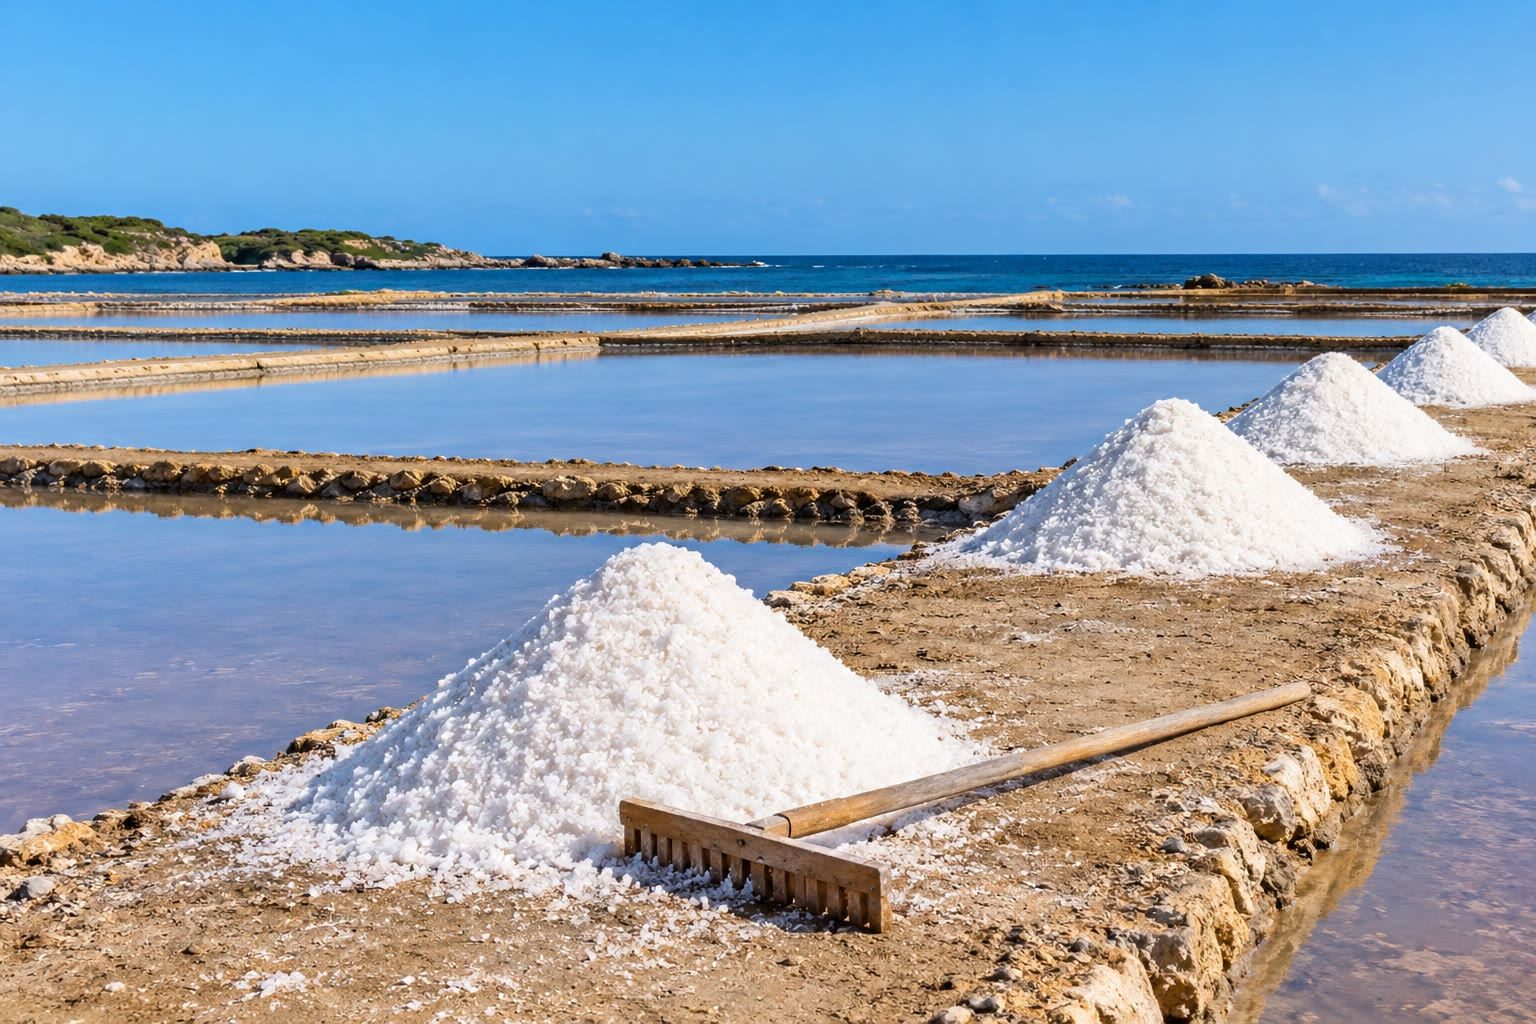
\includegraphics[width=0.62\linewidth]{images/book1/ai/g2-salt-pans.jpg}

{\small Zoutpannen aan zee: de zon laat het water opdrogen, het zout
blijft in witte hopen achter.}
\end{omfigure}

\begin{remark}[Oplossen is geen smelten]\label{rem:g2:mixing-and-dissolving:not-melting}
Mensen zeggen vaak dat suiker in de thee ``smelt''. Dat klopt niet:
smelten is wat een ijsblokje in de zon doet, het wordt vanzelf vloeibaar,
zonder dat er water bij nodig is. Suiker in thee heeft het water nodig,
en de suiker zit er nog in, verspreid. Het juiste woord is
\emph{\omterm{def:g2:mixing-and-dissolving:dissolve}{oplossen}}.
\end{remark}

\section{Oefeningen}

\begin{exercise}[$\star$]\label{exo:g2:mixing-and-dissolving:1}
Welke van deze vaste stoffen \omterm{def:g2:mixing-and-dissolving:dissolve}{lossen op} in water, en welke niet? Suiker,
zand, zout, krijt, kiezels.
\end{exercise}

\begin{exercise}[$\star$]\label{exo:g2:mixing-and-dissolving:2}
Wat is een \omterm{def:g2:mixing-and-dissolving:dissolve}{oplossing}? Geef twee voorbeelden uit dit hoofdstuk.
\end{exercise}

\begin{exercise}[$\star$]\label{exo:g2:mixing-and-dissolving:3}
Is een kom muesli een mengsel? Kun je elk van de delen nog zien?
\end{exercise}

\begin{exercise}[$\star$]\label{exo:g2:mixing-and-dissolving:4}
Iemand roert een wit poeder door een glas water. Na een paar minuten is
het water troebel en ligt er een wit laagje op de bodem. Is het poeder
opgelost? Leg uit met
\cref{met:g2:mixing-and-dissolving:test}.
\end{exercise}

\begin{exercise}[$\star$]\label{exo:g2:mixing-and-dissolving:5}
Een glas siroopwater is roze. Is het helder? Is het kleurloos? Is het
een \omterm{def:g2:mixing-and-dissolving:dissolve}{oplossing}?
\end{exercise}

\begin{exercise}[$\star$]\label{exo:g2:mixing-and-dissolving:6}
Na het roeren is er in een kopje thee geen suiker meer te zien. Geef de
aanwijzing die laat zien dat de suiker er nog is.
\end{exercise}

\begin{exercise}[$\star$]\label{exo:g2:mixing-and-dissolving:7}
Wat haalt de zon weg in de zoutpannen, en wat blijft er achter?
\end{exercise}

\begin{exercise}[$\star$]\label{exo:g2:mixing-and-dissolving:8}
Tom zegt: ``De suiker is in mijn thee gesmolten.'' Welk woord moet hij
gebruiken, en waarom?
\end{exercise}

\begin{exercise}[$\star\star$]\label{exo:g2:mixing-and-dissolving:9}
Kijk naar de figuur met de twee bekerglazen. Hoe zie je, zonder de
woorden eronder te lezen, in welk bekerglas het zand zit?
\end{exercise}

\begin{exercise}[$\star\star$]\label{exo:g2:mixing-and-dissolving:10}
Een druppel kraanwater droogt op een zwart bord op en laat een klein wit
kringetje achter. Wat vertelt dat ons over kraanwater?
\end{exercise}

\begin{exercise}[$\star\star$]\label{exo:g2:mixing-and-dissolving:11}
In het laboratorium heeft een docente twee glazen met een heldere,
kleurloze vloeistof: in het ene zit zuiver water, in het andere zout
water. Niemand mag ervan proeven. Hoe kan zij uitzoeken welk glas welk
is?
\end{exercise}
